\subsection{Expressiveness of \Nec Specifications}
\label{s:expressiveness}

Both the object capability literature and more recently the smart contract literature are rich sources for exemplars to try \Nec on. Ensuring that a visited web page cannot leak your confidential data was looked at by \citeauthor{dd}. It is interesting to see how straightforward it is to state assertions that protect the exemplars from attacks that have caused grief in the past.


\subsubsection{DOM}
\label{ss:DOM}

The key structure underlying a web browser is the Domain Object Model
(DOM), a recursive composite tree structure of objects that represent
everything display in a browser window.  Each window has a single DOM
tree which includes both the page's main content and also third party
content such as advertisements. To ensure third party content cannot
affect a page's main content,
specifications for attenuation for the DOM were proposed in
\textit{Devriese et al:}   \cite{dd}. 

This example deals with a tree of DOM nodes: Access to a DOM node
gives access to all its parent and children nodes, and the ability to
modify the node's properties. However, as the top nodes of the tree
usually contain privileged information, while the lower nodes contain
less crucial third-party information, we want to be able to limit  access given to third parties to only the lower part of the DOM tree. We do this through a \prg{Wrapper}, which has a field \prg{node} pointing to a \prg{Node}, and a field \prg{height} which restricts the range of \prg{Node}s which may be modified through the use of the particular \prg{Wrapper}. Namely, when you hold a \prg{Wrapper}  you can modify the \prg{property} of all the descendants of the    \prg{height}-th ancestors of the \prg{node} of that particular \prg{Wrapper}. It is not difficult to write such a \prg{Wrapper}; a possible implementation  appears in Figure \ref{fig:DOM}.
\begin{figure}[htb]
\begin{tabular}{llll}
\ \ &
\begin{minipage}{0.45\textwidth}
\begin{lstlisting}
method usingWrappers(unknwn){
   n1=Node(null,"fixed"); 
   n2=Node(n1,"robust"); 
   n3=Node(n2,"const"); 
   n4=Node(n3,"volatile");
   n5=Node(n4,"variable");
   n6=Node(n5,"ethereal");
   w=Wrapper(n5,1);
   
   unknwn.untrusted(w);
   
   assert n2.property=="robust" 
   ...
}
\end{lstlisting}
\end{minipage}
& & 
\begin{minipage}{0.75\textwidth}
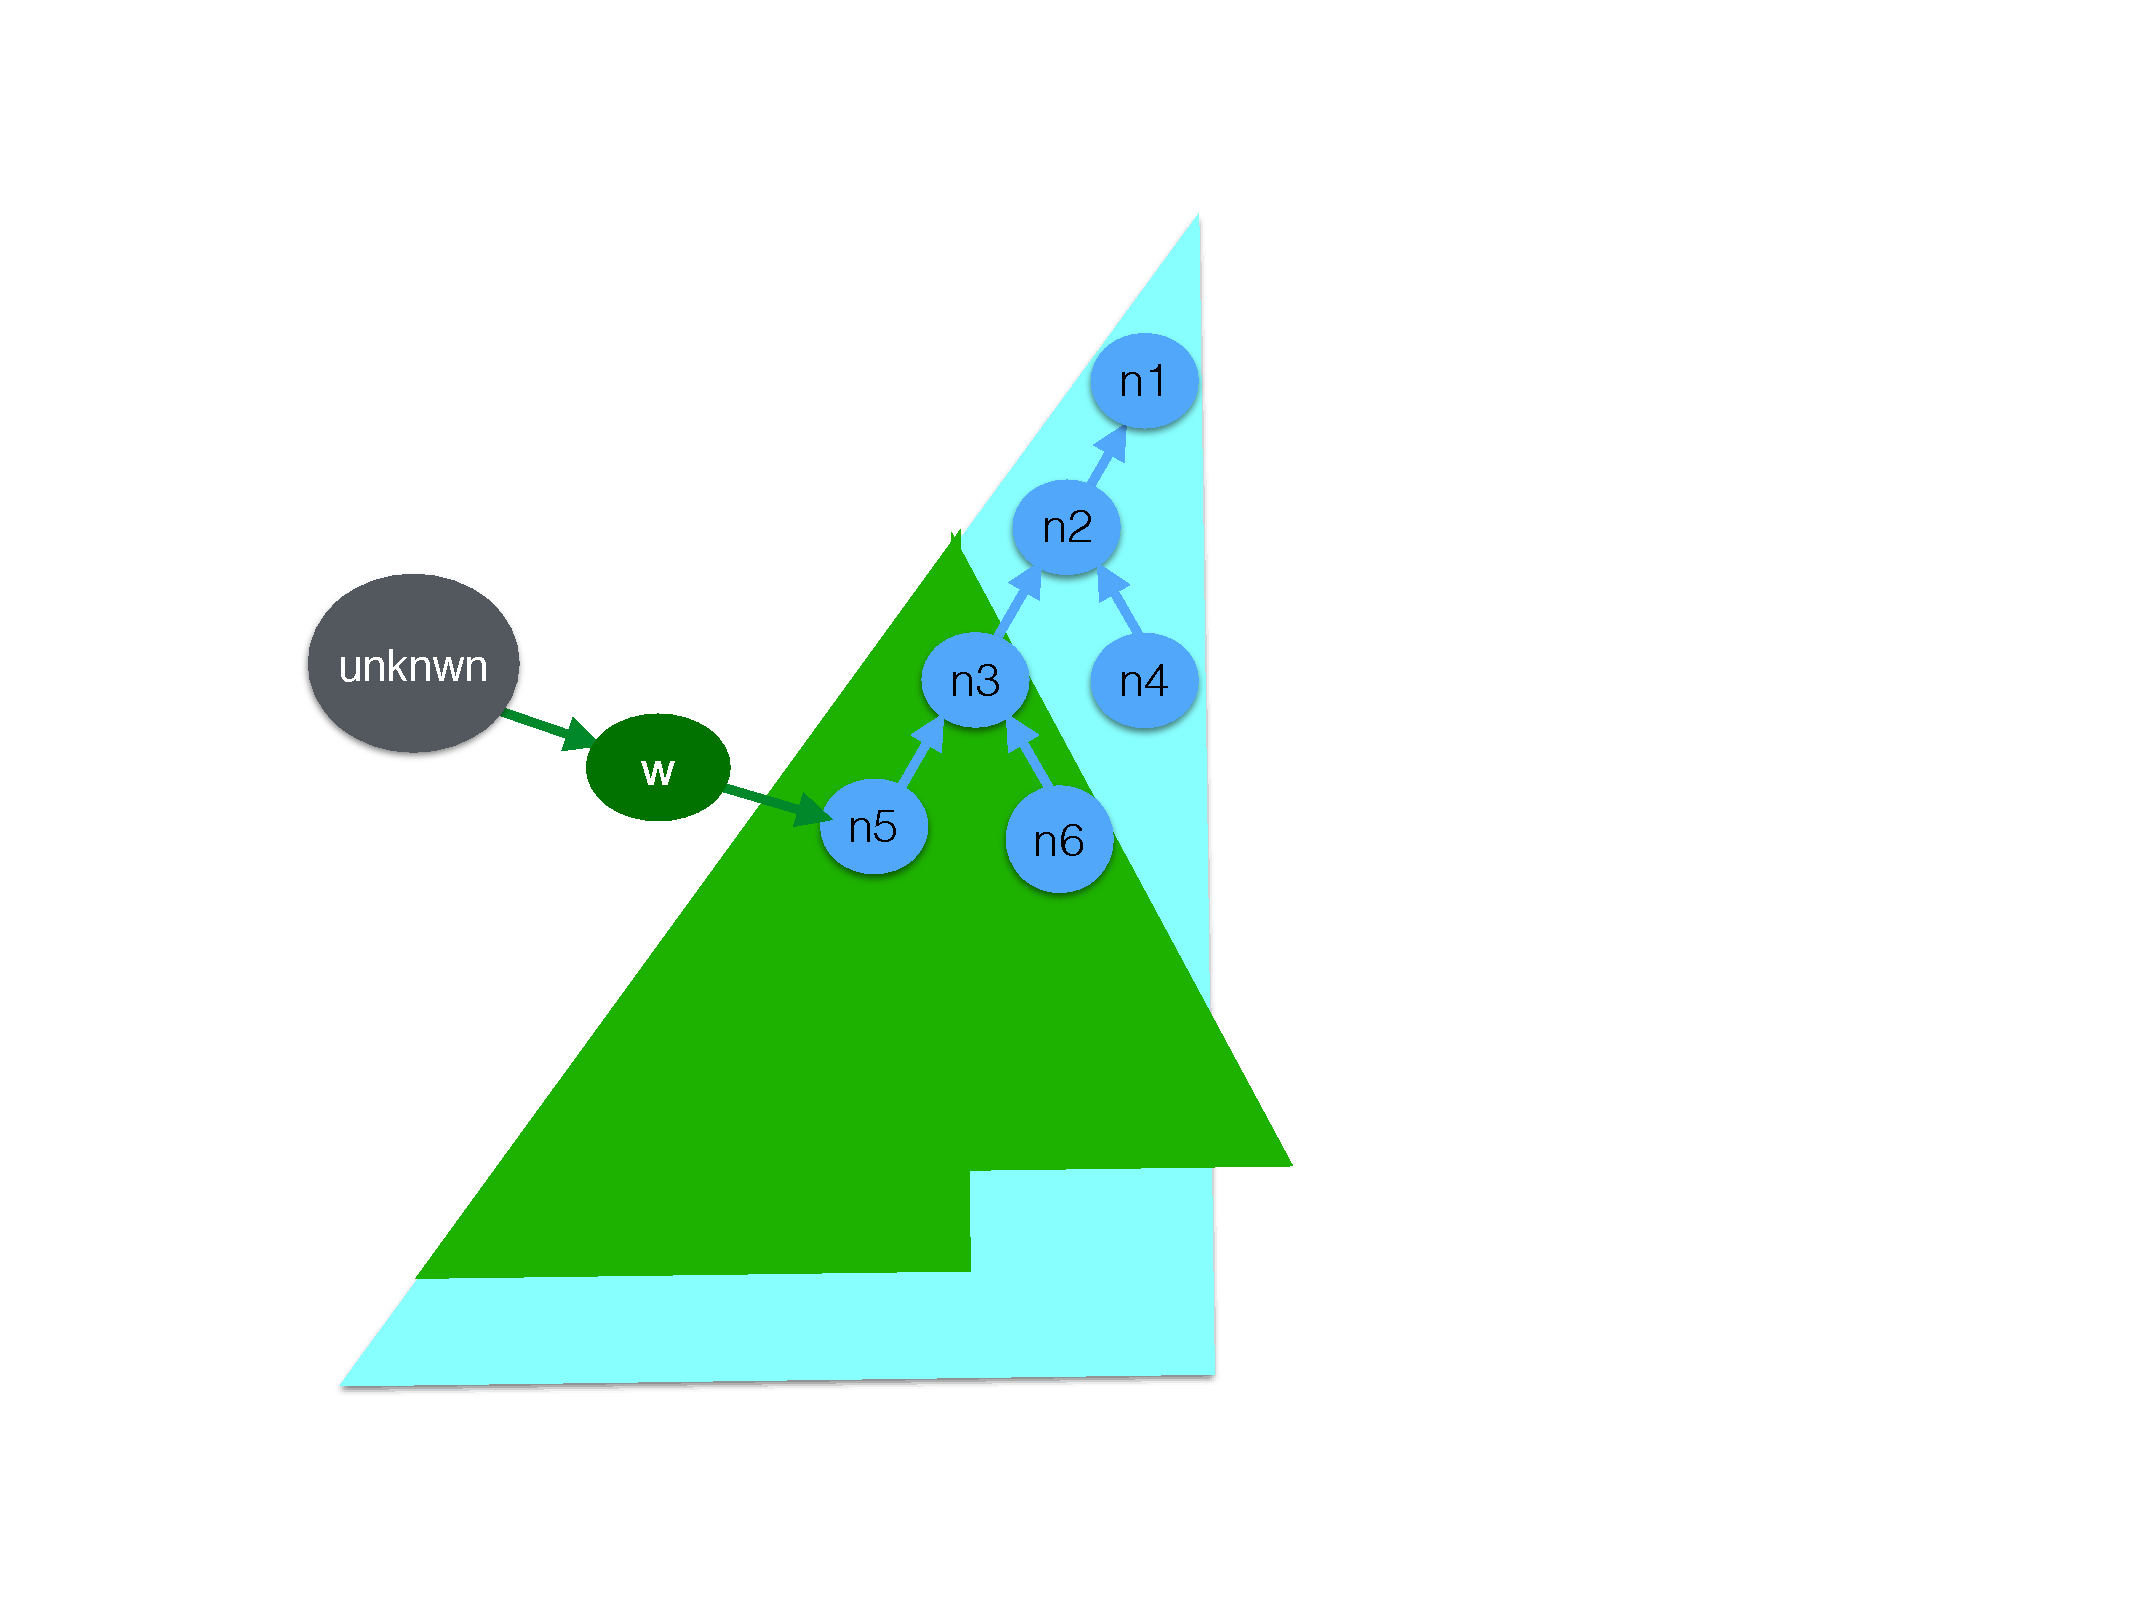
\includegraphics[width=\linewidth, trim=145  320 60 105,clip]{diagrams/DOM.pdf}
\strut \\
\strut \\

\end{minipage}
\end{tabular}
 \vspace*{-4.5mm}
\caption{\prg{Wrapper}s protecting \prg{Node}s from~\cite{FASE}}
\label{fig:DOM}
\end{figure}
In  Fig. \ref{fig:DOM}, a wrapper \prg{w} is defined, wrapping node \prg{n5}, with 
height \prg{1}. This provides \prg{unknwn} (some unknown client object) the capability to modify 
properties of \prg{n5}, and any nodes \prg{1} layer above and any of their descendants (i.e. node \prg{n3} and \prg{n6}), but no more.



\prg{DOMSpec} states that if the property of a node in a DOM tree changes,
it follows that either some non-node, non-wrapper object presently has 
access to a node of the DOM tree, or to some wrapper with access to some 
ancestor of the node that was modified.
\begin{lstlisting}[language = Chainmail, mathescape=true, frame=lines]
DOMSpec $\triangleq$ from nd : Node $\wedge$ nd.property = p
            to nd.property != p
            onlyIf $\exists$ o.[$\neg$ o : Node $\wedge$ $\neg$ o : Wrapper $\wedge$ 
                        ($\exists$ nd' : Node.[$\access{\prg{o}}{\prg{nd'}}$] $\vee$ 
                         $\exists$ w : Wrapper, k : $\mathbb{N}$.[$\access{\prg{o}}{\prg{w}}$ $\wedge$ nd.parnt$^{\prg{k}}$ = w.node.parnt$^{\prg{w.height}}$] )]
\end{lstlisting}

\subsubsection{ERC20}
The ERC20\cite{ERC20} is a widely used token standard describing the basic functionality of any Ethereum-based token 
contract. This functionality includes issuing tokens, keeping track of tokens belonging to participants, and the 
transfer of tokens between participants. Tokens may only be transferred if there are sufficient tokens in the 
participant's account, and if either they (using the \prg{transfer} method) or someone authorized by the participant (using the \prg{transferFrom} method) initiated the transfer. 

We specify these necessary conditions here using \Nec. Firstly, \prg{ERC20Spec1} 
says that if the balance of a participant's account is ever reduced by some amount $m$, then
that must have occurred as a result of a call to the \prg{transfer} method with amount $m$ by the participant,
or the \prg{transferFrom} method with the amount $m$ by some other participant.
\begin{lstlisting}[language = Chainmail, mathescape=true, frame=lines]
ERC20Spec1 $\triangleq$ from e : ERC20 $\wedge$ e.balance(p) = m + m' $\wedge$ m > 0
              nxt e.balance(p) = m'
              onlyIf $\exists$ p' p''.[$\calls{\prg{p'}}{\prg{e}}{\prg{transfer}}{\prg{p, m}}$ $\vee$ 
                     e.allowed(p, p'') $\geq$ m $\wedge$ $\calls{\prg{p''}}{\prg{e}}{\prg{transferFrom}}{\prg{p', m}}$]
\end{lstlisting}
Secondly, \prg{ERC20Spec2} specifies under what circumstances some participant \prg{p'} is authorized to 
spend \prg{m} tokens on behalf of \prg{p}: either \prg{p} approved \prg{p'}, \prg{p'} was previously authorized,
or \prg{p'} was authorized for some amount \prg{m + m'}, and spent \prg{m'}.
\begin{lstlisting}[language = Chainmail, mathescape=true, frame=lines]
ERC20Spec2 $\triangleq$ from e : ERC20 $\wedge$ p : Object $\wedge$ p' : Object $\wedge$ m : Nat
              nxt e.allowed(p, p') = m
              onlyIf $\calls{\prg{p}}{\prg{e}}{\prg{approve}}{\prg{p', m}}$ $\vee$ 
                     (e.allowed(p, p') = m $\wedge$ 
                      $\neg$ ($\calls{\prg{p'}}{\prg{e}}{\prg{transferFrom}}{\prg{p, \_}}$ $\vee$ 
                              $\calls{\prg{p}}{\prg{e}}{\prg{allowed}}{\prg{p, \_}}$)) $\vee$
                     $\exists$ p''. [e.allowed(p, p') = m + m' $\wedge$ $\calls{\prg{p'}}{\prg{e}}{\prg{transferFrom}}{\prg{p'', m'}}$]
\end{lstlisting}

\subsubsection{DAO}
The Decentralized Autonomous Organization (DAO)~\cite{Dao}  is a well-known Ethereum contract allowing 
participants to invest funds. The DAO famously was exploited with a re-entrancy bug in 2016, 
and lost \$50M. Here we provide specifications that would have secured the DAO against such a 
bug. \prg{DAOSpec1} says that no participant's balance may ever exceed the ether remaining 
in DAO.
\begin{lstlisting}[language = Chainmail, mathescape=true, frame=lines]
DAOSpec1 $\triangleq$ from d : DAO $\wedge$ p : Object
            to d.balance(p) > d.ether
            onlyIf false
\end{lstlisting}
Note that \prg{DAOSpec1} enforces a class invariant of \prg{DAO}, something that could be enforced
by traditional specifications uing class invariants.
The second specification \prg{DAOSpec2} states that if after some single step of execution, a participant's balance is \prg{m}, then 
either 
\begin{description}
\item[(a)] this occurred as a result of joining the DAO with an initial investment of \prg{m}, 
\item[(b)] the balance is \prg{0} and they've just withdrawn their funds, or 
\item[(c) ]the balance was \prg{m} to begin with
\end{description}
\begin{lstlisting}[language = Chainmail, mathescape=true, frame=lines]
DAOSpec2 $\triangleq$ from d : DAO $\wedge$ p : Object
            nxt d.balance(p) = m
            onlyIf $\calls{\prg{p}}{\prg{d}}{\prg{repay}}{\prg{\_}}$ $\wedge$ m = 0 $\vee$ $\calls{\prg{p}}{\prg{d}}{\prg{join}}{\prg{m}}$ $\vee$ d.balance(p) = m
\end{lstlisting}
